\documentclass{article} % Oder eine andere Dokumentklasse wie report, book, etc.
\usepackage[utf8]{inputenc} % Bestimmt die Eingabe-Kodierung
\usepackage[T1]{fontenc} % Bestimmt die Ausgabe-Kodierung
\usepackage{graphicx}
\usepackage{amsmath}
\usepackage{hyperref}


\begin{document}
	
	\title{Deep Reinforcement Learning Group Project}
	\maketitle
	
	Group:
	\begin{itemize}
		\item Marvin Kohnen
		\item Moritz Gehring
		\item Julius Ferber 
		
	\end{itemize}
	
	Code and results can be found at \url{https://github.com/MarvinKohnen/deep-reinforcement-learning/tree/main/drl_deep_project}.
	\section{Exercise A}
	
	\subsection{Basic Training Routine: DQN} 
	We first implemented a DQN agent, given the full state space on the classic tournament map. Furthermore, we adjusted the existing q\_learning file with our own values. After mutliple iterations, the best performing model ran with the following values and rewards: \newline

	Model stats: 
	\begin{itemize}
		\item $\epsilon$ start at 1
		\item $\epsilon$ end at 0.05
		\item $\epsilon$ exponential epsilon decay of 100.000 
		\item $\gamma$ is 0.99
		\item 50.000 episodes
	\end{itemize}
	
	Rewards:
	\begin{itemize}
		\item  COIN\_COLLECTED: 1
		\item KILLED\_SELF: -5
		\item INVALID\_ACTION: -0.5
		\item KILLED\_OPPONENT: 5
		\item CRATE\_DESTROYED: 0.1
		\item GOT\_KILLED: -5
		\item WAITED: -0.1
	\end{itemize}
		
	 The model showed signs of learning (as can be seen in Figure \ref{fig:1} rewards (top) and episode length (bottom)). When running the model, this learning manifests in the agent moving in corners to increase survival rate, while neglecting coin collection, crate destruction or aggression towards other players. Moreover, the model is quite unstable, often self-killing the agent rather early on during the run. 
	
	\begin{figure}[h!]
		\centering
		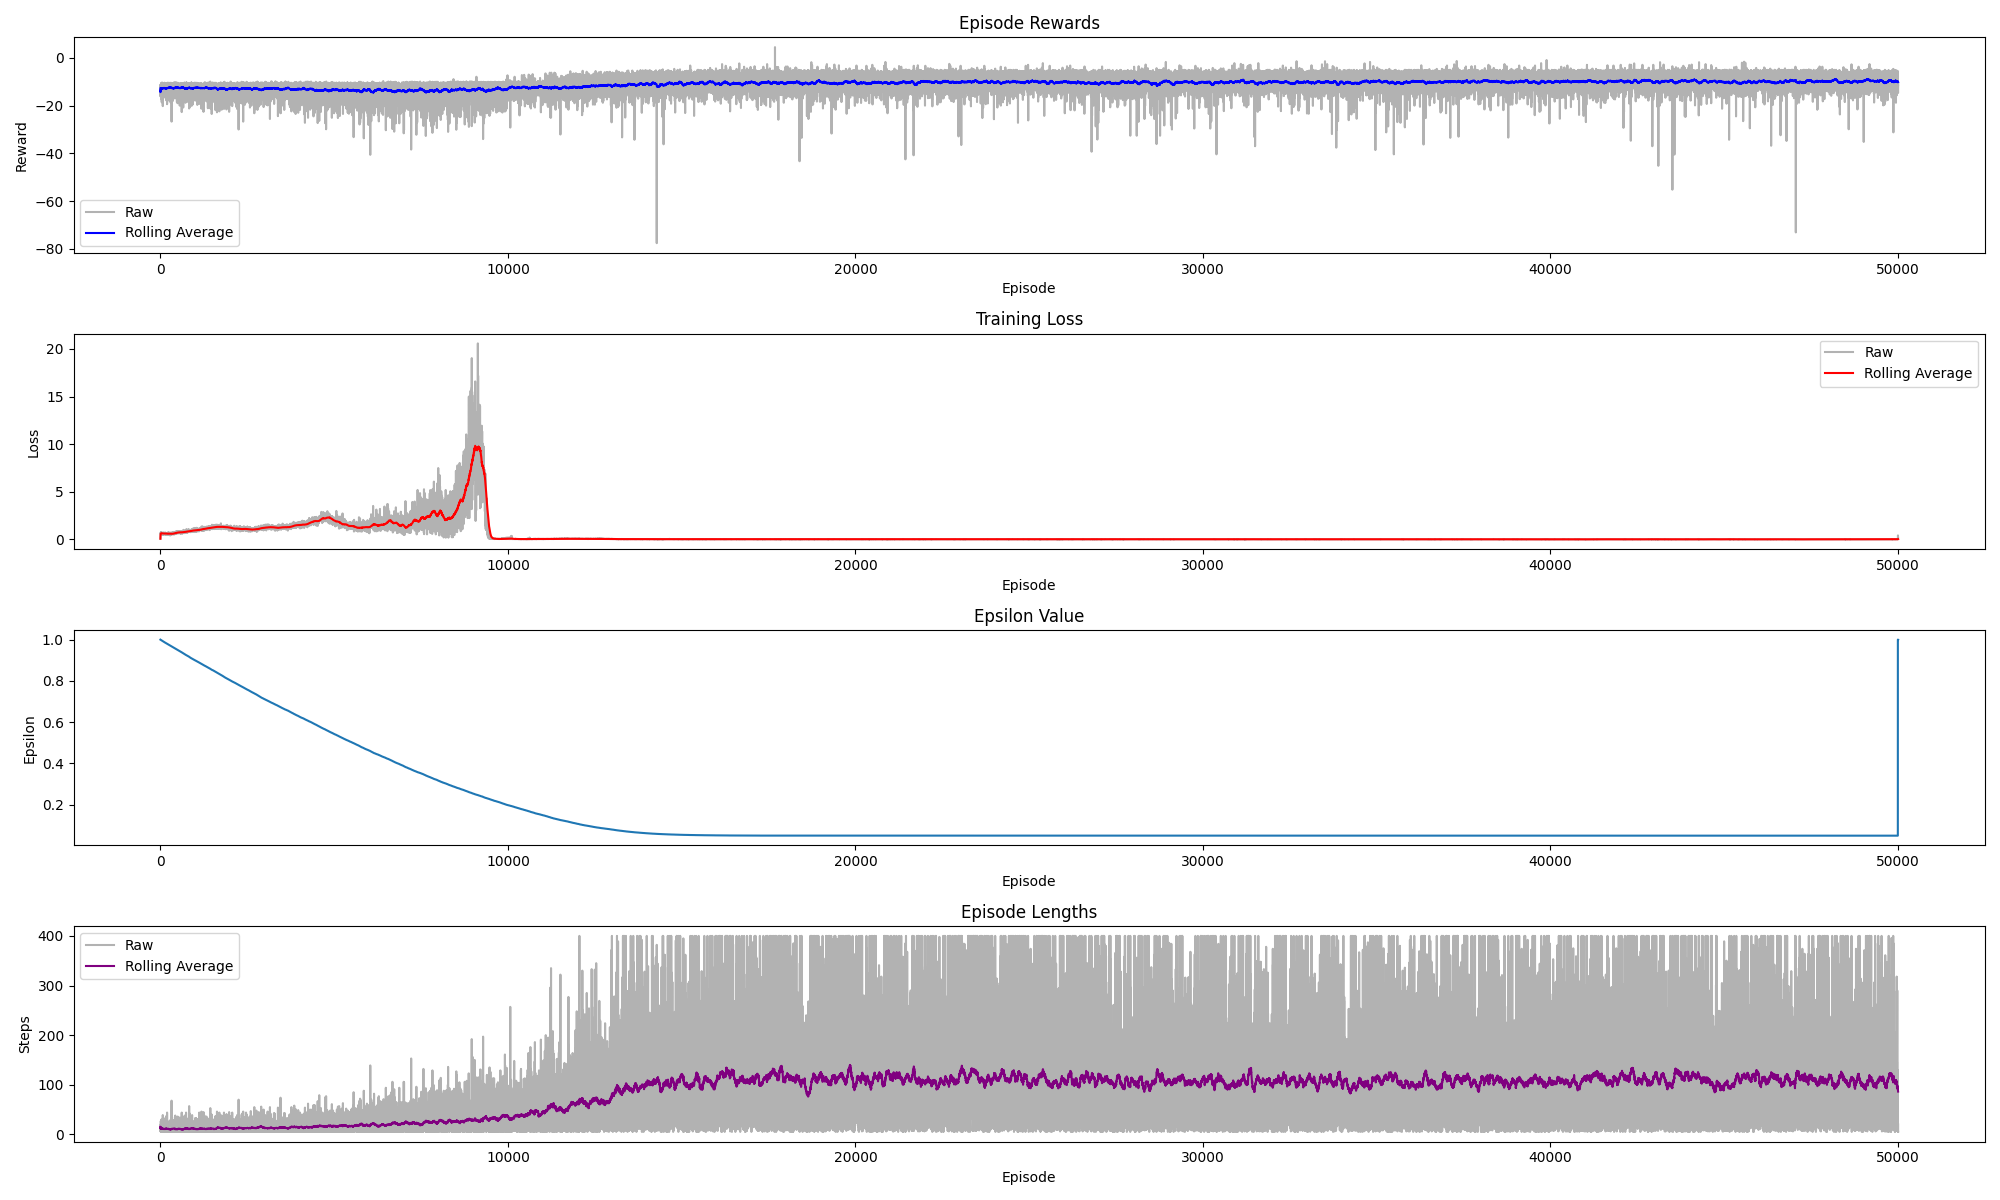
\includegraphics[width=1.0\textwidth]{images/first_training_results}
		\caption{Results of simple DQN Training, plots for reward, training loss, epsilon decay, and episode length over 50000 Episodes}
		\label{fig:1}
	\end{figure}
	
	
	The Code for this model is found in the folder EDIT HERE!!!!!!!!!!!!!!!!
	\newpage
	
	\section{Exercise B}
	\subsection{Reward Shaping}
	Our first approach to improve the DQN was to use different rewards, as this is the easiest way to influence the model behaviour. We realised, that the event KILLED\_SELF and GOT\_KILLED would punish our agent twice. Therefore we dropped the former from our reward structure. Furthermore, we increased the reward for coin collection and also introduced a reward for coin found and crate destroyed. Ultimately, these were the specific values that resulted in the best outcome:\newline
	
	Rewards:
	\begin{itemize}
		\item COIN\_COLLECTED: 2
		\item INVALID\_ACTION: -0.5
		\item KILLED\_OPPONENT: 5
		\item CRATE\_DESTROYED: 1
		\item GOT\_KILLED: -5
		\item WAITED: -0.1
		\item COIN\_FOUND: 1
	\end{itemize}
	
	
	\subsection{Curriculum Learning and Catastrophic Forgetting}
	We implemented various approaches to curriculum learning in our project. As stated earlier, our model was initially trained on the full tournament map, but we subsequently experimented with reduced-scale environments (e.g., 7x7 or 9x9 grids) to simplify the learning process. However, the models trained on these smaller maps failed to scale to larger environments, even when the scenario remained unchanged, rendering this approach ineffective.
	
	Our next strategy involved developing less complex scenarios within a 17x17 grid, which is equivalent in size to the tournament map. These simplified scenarios proved to be more approachable, allowing for faster training and yielding promising outcomes (as illustrated in Figure \ref{fig:3}, shwoing the curriculum coin scenario).
	
	Nevertheless, we encountered a significant challenge: when attempting to transfer the weights learned from these simpler scenarios to more complex environments (such as the curriculum-crate scenario or the full tournament map), we observed a case of - what we assume is - catastrophic forgetting. The model appeared to lose its previously acquired skills and struggled to perform tasks that were less demanding than those it had just learned.
	
	This issue remained unresolved despite our best efforts.
	
	\begin{figure}[h!]
		\centering
		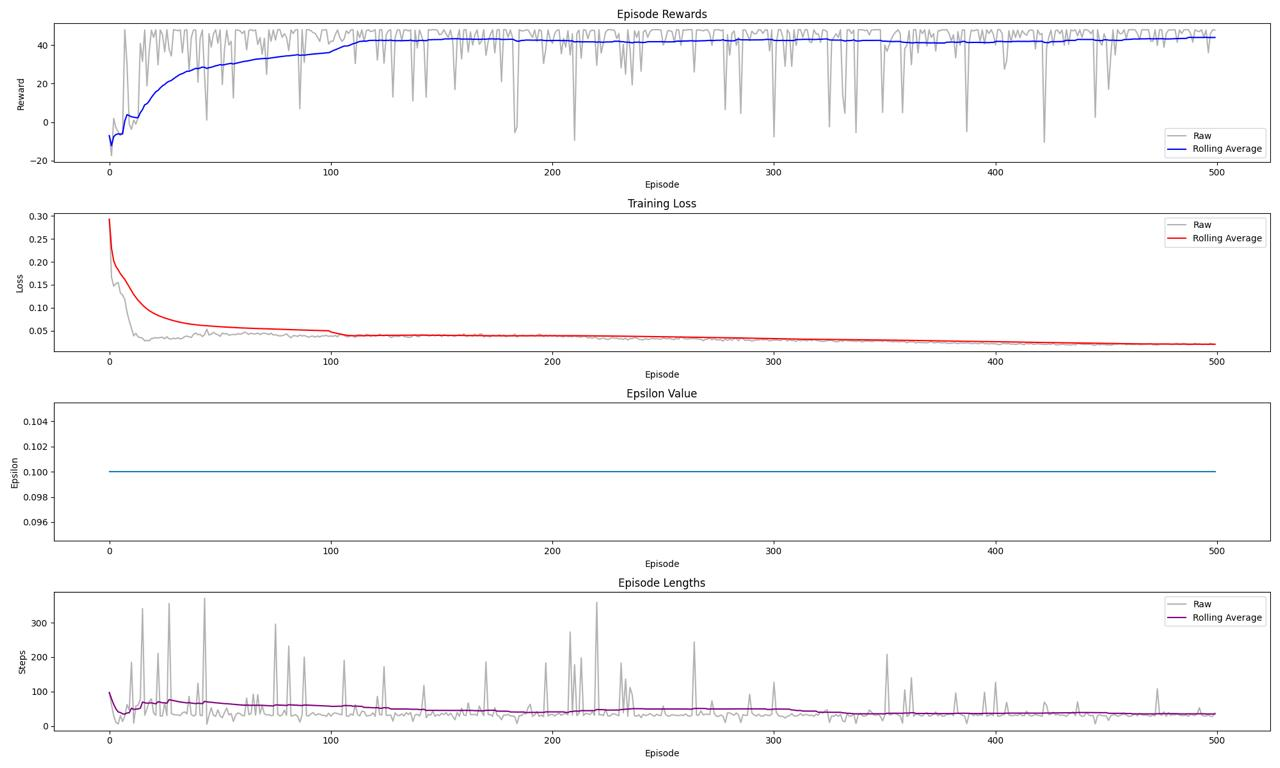
\includegraphics[width=1.0\textwidth]{images/curriculum_coin}
		\caption{Results for curriculum coin training. Only few trainings episodes were needed, with a relatively small (and constant) $\epsilon$ of 0.1}
		\label{fig:3}
	\end{figure}
	
	\subsection{Prioritized Experience Replay}
	Prioritized Experience Replay (PER) enhances our agent's learning by strategically sampling important experiences more frequently during training. Instead of uniform sampling, PER assigns priorities based on TD errors, effectively measuring how "surprising" or "unexpected" an experience was. This is particularly valuable in Bomberman, where critical moments like deaths, coin collection, and bomb encounters are rare but crucial for learning. These experiences typically generate larger TD errors, resulting in higher sampling priorities and more frequent replay. Our implementation uses a binary sum tree structure for efficient O(log n) priority-based sampling. New experiences initially receive maximum priority to ensure exploration, and their priorities are then updated based on their TD errors using the formula priority
	\begin{equation}
		(|TD\_error| + \varepsilon)^{\alpha}
	\end{equation}
	
	To correct the bias introduced by non-uniform sampling, we use importance sampling weights. The system is tuned with $\alpha$=0.6 for prioritization strength, $\beta$ starting at 0.4 and annealing to 1.0 for bias correction, and $\epsilon$=0.01 to ensure non-zero priorities.\footnote{The implementation and the hyperparameters were taken from the paper \url{https://arxiv.org/pdf/1511.05952}}
	
	
	\subsection{Model Improvement}
	After an initial size of the network with two hidden layers of size 64, we later changed the size of the first hidden layer to 128, since the number of inputs rose to 80. This change was made based on the heuristic described in the information bottleneck theory, which roughly states, that the representation space should first be expanded (80 $\rightarrow$ 128) and then compressed (128 $\rightarrow$ 64) for optimal deep learning. For further detail, one could use \url{https://arxiv.org/pdf/1503.02406} as a starting point.
	
	Another big change we only made near the end of the project was the reduction of $\gamma$ from 0.99 to 0.8. This resulted in much quicker and more stable learning on easier maps, but also to noticeable improvements on the classic tournament map. We presume this is the case, because in the TD update, the lower $\gamma$ corresponds to a lower impact of the q-values and therefore a higher impact of the reward, which in turn makes reward shaping more influential to the training.
	
	Another nob we tried to turn throughout the whole process was the epsilon value. In the end, our observations are the following: For smaller or simpler maps with a clear goal or a laid out path (like curriculum-coin), it seems like a small constant epsilon (like 0.1) leads to the most stable and fast learning, whereas on maps with a high degree of variability, a longer epsilon decay starting from a high value (like 0.9) going down to a low value (like 0.1) leads to a more broad understanding of possible situations, since the exploration phase is longer. We observed that training the last 1/4 of the time on the lower epsilon further helped refine the action selection for the beginning phase of an episode, after having learned goo q-values during the exploration phase.
	
	\subsection{Double DQN}
	We implemented a double DQN along the proposition in the Learnweb, but it did achieve worse results (see Figure \ref{fig:2}) and took noticeably more time to train in comparison to a DQN. Therefore it was not reasonably trainable in the given time frame. Since DQN usually struggles with maximation bias, we thought double DQN could help. As Bomberman is an environment with relatively sparse positive rewards, there are more pressing issues and better opitmizations at hand that we decided to try. 
	We dropped the approach because of these aforementioned reasons. Yet the code is still part of the repository.
	
	\begin{figure}[h!]
		\centering
		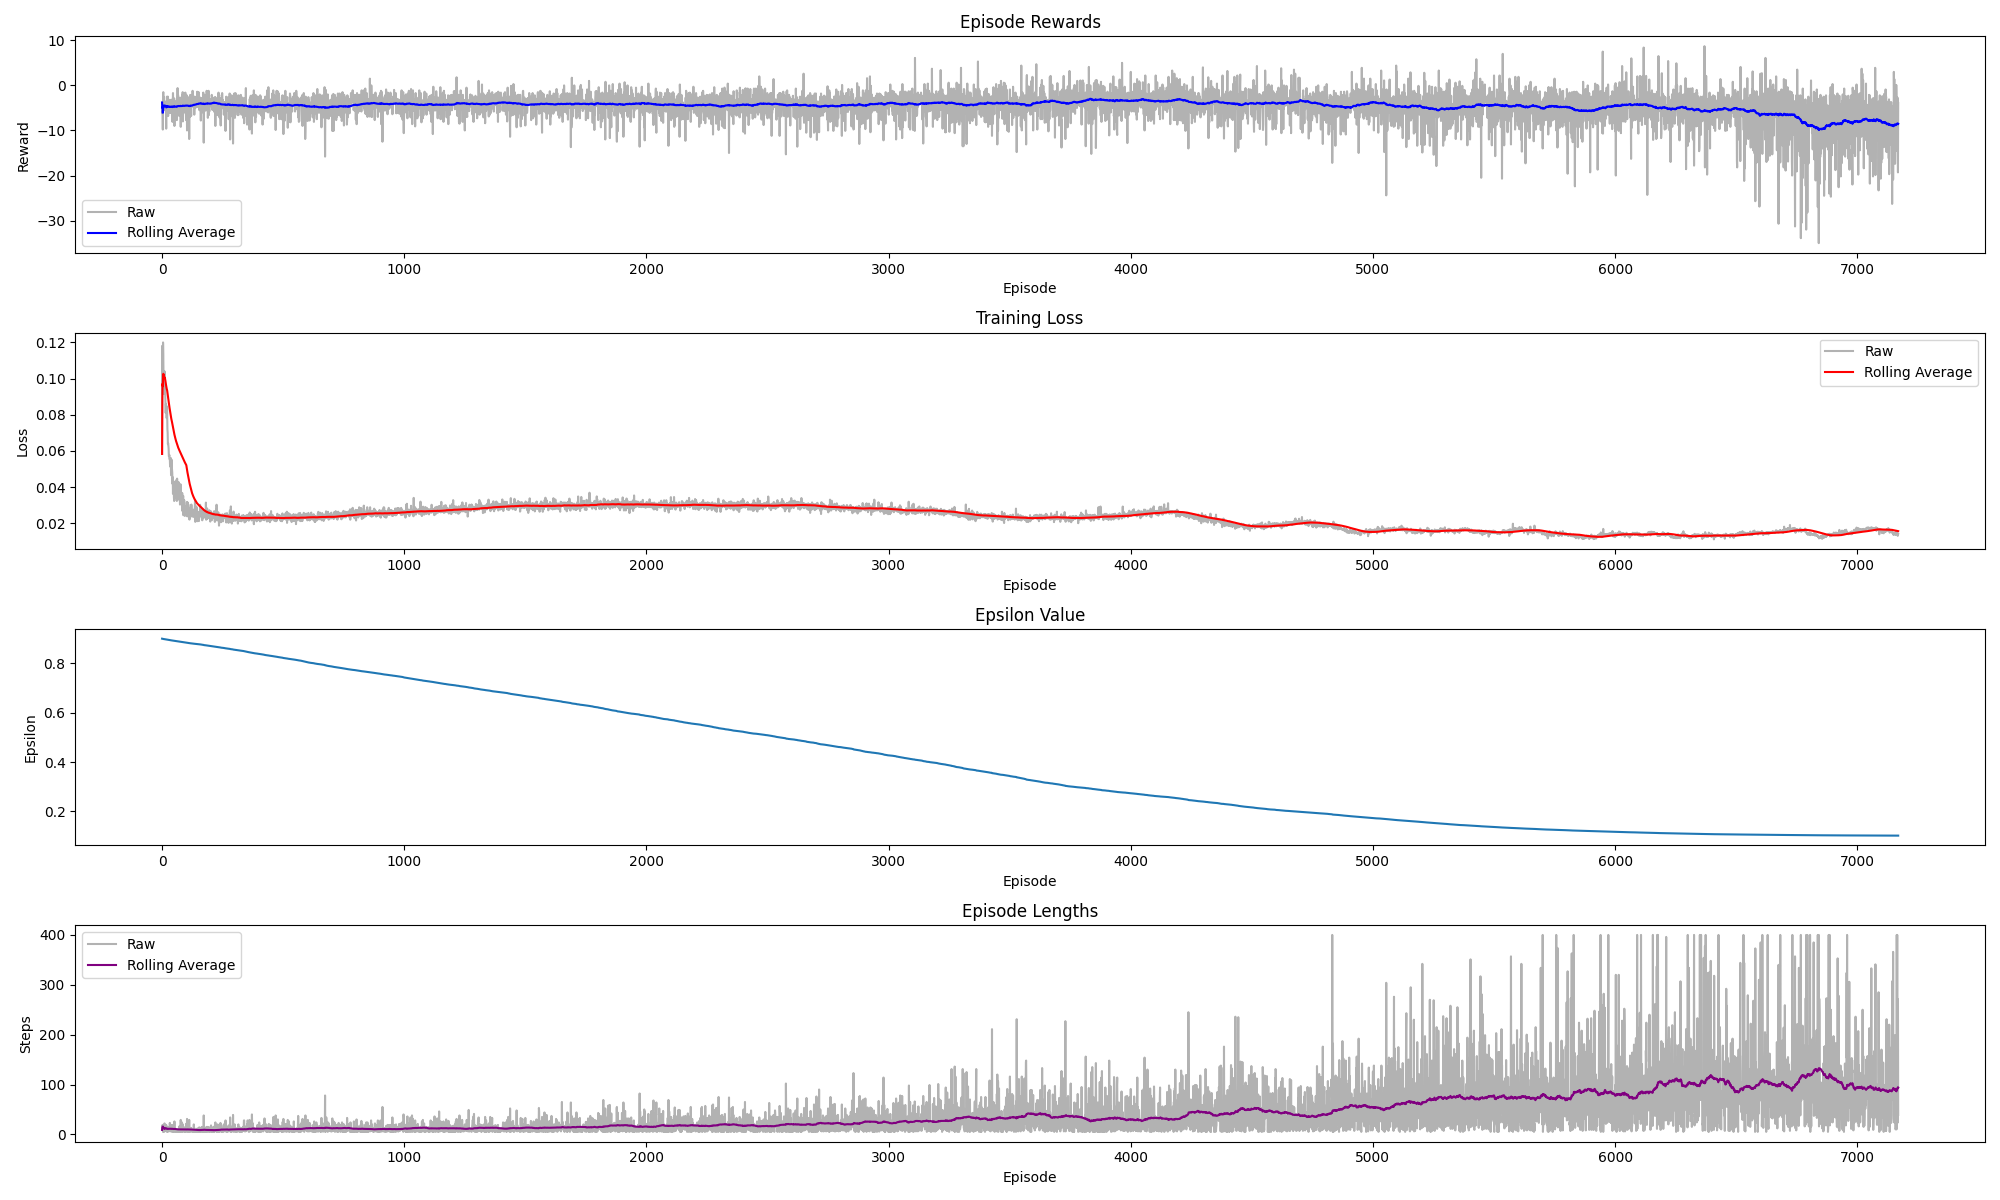
\includegraphics[width=1.0\textwidth]{images/double_dqn_results}
		\caption{Results of Double DQN Training, plots for reward, training loss, epsilon decay, and episode length over 7000 Episodes}
		\label{fig:2}
	\end{figure}
	
	\newpage
	
	\subsection{State Space Abstraction}
	After training the vanilla model on the full state space given by the environment, we could tell that the full state space was too large to efficiently train the agent. Therefore we tried to reduce the input by restricting our state space using a single padded 7x7 window of a „scope representation“ we had implemented for the rule-based-agent. The representation used breadth-first search to make a single array showing the different features like crates, coins or bombs with their own values each, and assigning a value to all the cells the agent could possibly move to without a blockade. This representation did not work very well though, since the network could not interpret the different values and the representation was not invariant with respect to the starting position. 
	Our next approach worked better by using more relational inputs rather than a direct representation of the grid. This meant we used 8 inputs for the immediate surrounding cells, categorizing them into walkable and unwalkable, 16 inputs for the closest object in each direction, and 8 global features like the distance of the nearest coin, bomb and enemy for a total of 32 features. This change boosted performance significantly, while still remaining quite small in size. 
	Our final enhanced representation extended this approach by adding 40 features for danger detection for all 8 directions, which included checking the bomb timer of each bomb in the surrounding cells. Some small changes were made to the existing abstraction, which resulted in a total of 80 input features. This once again boosted performance, especially in dodging bombs, but still remains faulty in certain cases.
	
	\subsection{State Space Transformation}
	\subsubsection{Inspiration}
	\begin{itemize}
		\item The agent's position in the map does not affect the possible actions.
		\item The agent's position in the map does not significantly affect the optimal action.
		\item Example:
		\begin{itemize}
			\item The agent is in the top left quadrant.
			\item The optimal action is to move to the right.
			\item If the map was mirrored along its vertical axis (including the agent's position), the optimal action would therefore be to move to the left.
			\item However, the state representation/observation is different in the mirrored case.
			\item Even though the optimal action is virtually the same (just mirrored).
		\end{itemize}
		\item Conclusion: If we can ensure that the agent is only learning on any one quadrant, and only observes states where it is in that same quadrant, variance is reduced.
	\end{itemize}
	
	\subsubsection{Idea}
	
	\begin{itemize}
		\item We transform the state space to only portray the agent in the top left quadrant:
		\begin{itemize}
			\item If the agent is in any other quadrant, the matrix (numpy array) is flipped (mirrored) to place the agent in the top left quadrant.
			\item If the agent walks across the halfway line either to the right or the bottom, the transformation is adapted dynamically: The agent ``thinks'' that it ``bounced off'' at the halfway line.
			\item The actions are transformed accordingly: left $\leftrightarrow$ right, up $\leftrightarrow$ down.
		\end{itemize}
		\item In theory, this should cut the state space by 3/4, without losing any information:
		\begin{itemize}
			\item The whole state is still represented (just mirrored).
			\item As there is no information tied specifically to the quadrant the agent is in, the transformation has no information loss.
			\item Overfitting should not be an issue, as \textbf{all} input states have the agent in the top left quadrant (because all observed states are transformed before input).
		\end{itemize}
	\end{itemize}
	
	\subsubsection{Results}
	
	\begin{itemize}
		\item Due to an implementation error that did not show up easily in debugging, the state transformation did not work correctly in the beginning, nullifying its results before the error was caught.
		\item In the few runs after fixing that error, no discernible effect could be seen. We believe this is due to multiple reasons:
		\begin{itemize}
			\item Most of the refined state abstractions used do not take much of the original state arrays into account immediately, instead using only the immediate surroundings and then calculating relative positions.
			\begin{itemize}
				\item While this should still be stabilised by the transformation (e.g. the relative distance of the next wall to the left is likely in a narrower range), the effect is not as significant as when using e.g. the entire arrays for walls, bombs, etc.
				\item Input features such as the distance to the nearest coin is not at all affected by the transformation, as the distance between 2 points in the map is invariant to any transformations.
			\end{itemize}
			\item Even though all observations have the agent in the top left quadrant, this might still lead to overfitting in some way, especially with the more refined state abstractions and the relative positions.
		\end{itemize}
	\end{itemize}
	
	
	
\end{document}